\section{Results on the development sets}
\label{sec:results}
\FloatBarrier

\begin{table}[t]
  \centering
  \caption{Zero-shot top-1 agreement (\%) with high-win-rate players,
  deployment mode, forced picks included; 95\% cluster-bootstrap
  confidence intervals over drafts in parentheses. Sets: The Brothers'
  War (BRO), Teenage Mutant Ninja Turtles (TMT), Secrets of Strixhaven
  (SOS), and Marvel Super Heroes (MSH). F-full's dev-trio cells are never
  quoted, since it trains on those three sets.}
  \label{tab:main}
  \footnotesize
  \setlength{\tabcolsep}{2.4pt}
  % The CI columns make this a hair wider than \textwidth; center the
  % overhang symmetrically instead of letting it spill into one margin.
  \makebox[\textwidth][c]{% AUTO-GENERATED by scripts/make_paper_tables.py -- do not edit.
% Main results: expert-slice deployment-mode top-1 (95% cluster-bootstrap CIs over drafts).
\begin{tabular}{lccccc}
\toprule
Model & BRO & TMT & SOS & Dev mean & MSH \\
\midrule
DraftFM (F-dev, zero-shot) & 48.9 {\scriptsize(48.8, 49.0)} & 57.5 {\scriptsize(57.3, 57.7)} & 56.5 {\scriptsize(56.4, 56.6)} & 54.3 & \pendingcell \\  % run=20260704_135822_f_dev; run=20260704_135822_f_dev; run=20260704_135822_f_dev; run=20260704_135822_f_dev; pending: eval
DraftFM (F-full, zero-shot) & -- & -- & -- & -- & \pendingcell \\  % pending: eval
\midrule
Per-set ceiling & 65.6 & 71.0 & 70.2 {\scriptsize(69.8, 70.6)} & 68.9 & \pendingcell \\  % run=perset-BRO-latest; run=perset-TMT-latest; run=perset-SOS-protocol-validation; pending: post-T0
\quad F-dev / ceiling (unaligned) & 0.745 & 0.810 & 0.805 & 0.787 & \pendingcell \\  % pending: post-T0
\bottomrule
\end{tabular}
}
\end{table}

\paragraph{Zero-shot transfer on the development trio.}
% Aligned normalized score (scripts/eval_normalized_score.py, inner-joined
% on identical (draft_id, pack, pick) so zero-shot and ceiling score the
% same picks -- a much smaller aligned subset than the unaligned ratio's
% full slice, since the ceiling model's val split is small): run=
% 20260704_135822_f_dev. BRO 0.7430 (CI 0.7363-0.7503, n=59,572 aligned
% picks), TMT 0.8132 (CI 0.8015-0.8251, n=17,261), SOS 0.8019 (CI
% 0.7960-0.8077, n=69,803), dev-mean 0.7860.
Table~\ref{tab:main} reports zero-shot transfer on the development trio.
F-dev, the recipe used for architecture and hyperparameter selection,
trains on \FdevPicks M picks from \FdevSets{} sets and is then evaluated
on three sets it has never seen a pick from, where it agrees with
high-win-rate players on \FdevDevMean\% of picks. Every number in this
paragraph is a dev-trio rehearsal by the protocol's own design; the
paper's headline is the frozen MSH result of \S\ref{sec:msh}. Broken out
per set, DraftFM reaches \FdevBro\% / \FdevTmt\% / \FdevSos\% on BRO /
TMT / SOS. For comparison, a model trained directly on each of those
sets, the ceiling, reaches \CeilBro\% / \CeilTmt\% / \CeilSos\%.
DraftFM's pre-registered normalized score, its accuracy as a fraction of
that ceiling on identical held-out picks per \S\ref{sec:protocol}, is
\NormScoreBro\% / \NormScoreTmt\% / \NormScoreSos\%, with dev-mean
\NormScoreDevMean\%. A simpler, unaligned version of the same ratio,
taken over the full slice rather than the smaller aligned subset,
corroborates this on a much larger sample: \RatioBro\% / \RatioTmt\% /
\RatioSos\%, dev-mean \RatioDevMean\%. That unaligned ratio is not
itself the pre-registered metric, since the aligned version is capped by
the size of the ceiling model's own held-out split. Excluding forced
picks lowers the three numbers to \FdevBroNonForced\% /
\FdevTmtNonForced\% / \FdevSosNonForced\%. The deployment-mode skill
bucket selected on dev is the \DeployBucket{} win-rate bucket.

\paragraph{Reading the BRO row.}
BRO is the holdout on which \citet{bertram2024cards} report 55.4\%, the
strongest published unseen-set number. They reach it with card features,
learned image embeddings, and 16 usage statistics computed from human
play after the set's release, scored on all players rather than a
win-rate-filtered population. Our \FdevBro\% on the high-win-rate slice,
\FdevBroAllUsers\% on all players as the population-matched comparator,
is below that number, but the two are not a fair fight: their number
assumes information that does not exist on release day. The fair
comparison is against what the same paper achieves without post-release
usage statistics, 33.6--35.6\% on a single set, and every other
day-one-feasible baseline in Table~\ref{tab:baselines}. Against that
day-one bar, multi-set training on public card features closes most of
the distance to the usage-statistics number while using only release-day
information.

BRO is also the hardest set in the trio for transfer: its packs mix in a
63-card retro-artifact bonus sheet, examined directly in
\S\ref{sec:analysis}. Why TMT, the trio's licensed-IP set, nonetheless
transfers as well as SOS, and why BRO lags both, is analysed there too.
Figure~\ref{fig:tmt-tierlist} shows a real P1P1 bomb from TMT scored the
same way. For sets that are in the training corpus but have no dedicated
per-set model, the deployed system falls back to F-full's scoring;
Figure~\ref{fig:gallery} shows what that fallback looks like today for
LTR, LCI, and DMU.

\begin{figure}[t]
\centering
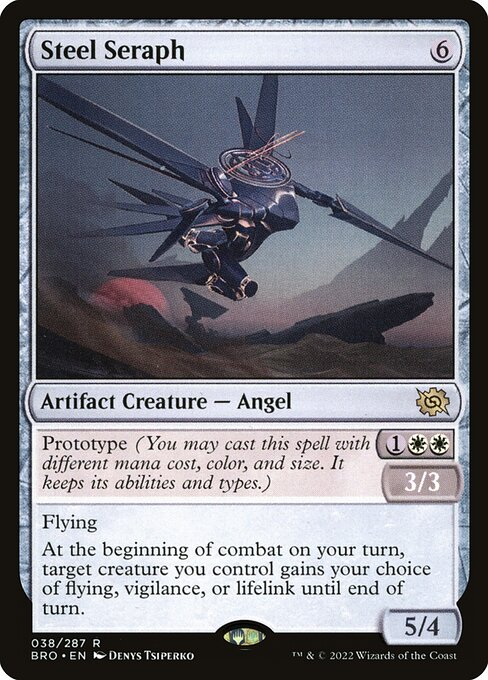
\includegraphics[width=0.24\linewidth]{figures/cards/steel-seraph.jpg}
\caption{Steel Seraph, BRO, the dev trio's hardest transfer set
(\S\ref{sec:analysis}). Real P1P1 expected value \VBroEv, the
\VBroPercentile{}th percentile of BRO's card pool by the deployed per-set
model's own ranking; the next two candidates in the pack,
\VBroRunnerOneName{} and \VBroRunnerTwoName{}, rank at the
\VBroRunnerOnePercentile{}th and \VBroRunnerTwoPercentile{}th. Percentile,
not a head-to-head split: Arena hides the pack between picks in this mode
(\S\ref{sec:arch}).}
\label{fig:bro-tierlist}
\end{figure}

\begin{figure}[t]
\centering

\includegraphics[width=0.24\linewidth]{figures/cards/april-oneil-hacktivist.jpg}
\caption{April O'Neil, Hacktivist, TMT, the dev trio's licensed-IP set
(\S\ref{sec:analysis}), a comic-book bomb the text encoder never saw
described in \mtg{} rules-text style. Real P1P1 expected value \VTmtEv,
the \VTmtPercentile{}th percentile of TMT's card pool.}
\label{fig:tmt-tierlist}
\end{figure}

\begin{figure}[t]
\centering
\begin{minipage}[b]{0.20\linewidth}
  \centering
  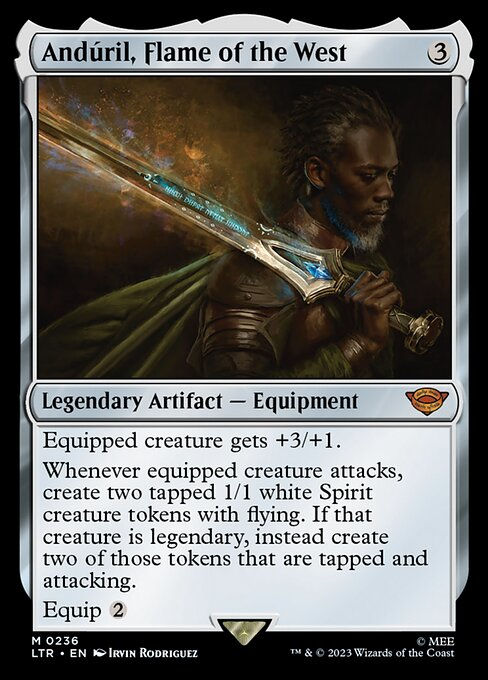
\includegraphics[width=\linewidth]{figures/cards/anduril-flame-of-the-west.jpg}\par
  \small LTR: EV \VGalLtrEv, pct \VGalLtrPercentile
\end{minipage}%
\hfill
\begin{minipage}[b]{0.20\linewidth}
  \centering
  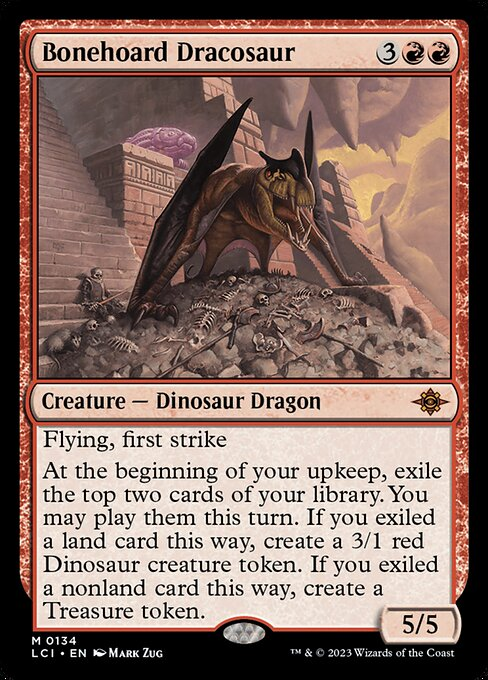
\includegraphics[width=\linewidth]{figures/cards/bonehoard-dracosaur.jpg}\par
  \small LCI: EV \VGalLciEv, pct \VGalLciPercentile
\end{minipage}%
\hfill
\begin{minipage}[b]{0.20\linewidth}
  \centering
  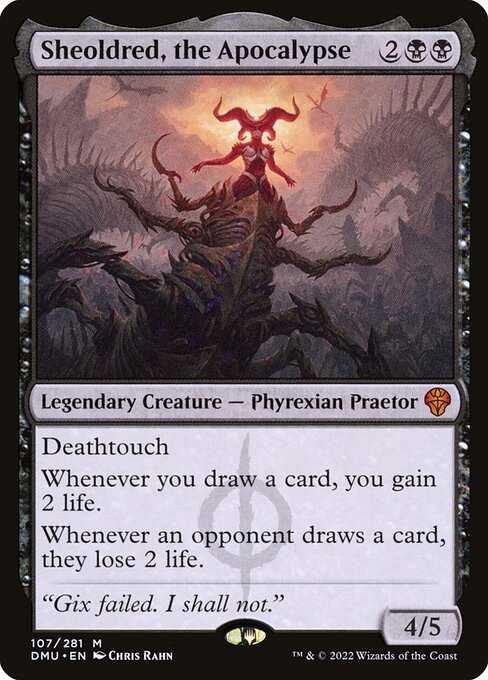
\includegraphics[width=\linewidth]{figures/cards/sheoldred-the-apocalypse.jpg}\par
  \small DMU: EV \VGalDmuEv, pct \VGalDmuPercentile
\end{minipage}
\caption{Three sets with no dedicated per-set model: The Lord of the
Rings: Tales of Middle-earth (LTR), The Lost Caverns of Ixalan (LCI),
and Dominaria United (DMU), all in F-full's 31-set training corpus.
Expected values and percentiles are computed as in
Figures~\ref{fig:bro-tierlist} and \ref{fig:tmt-tierlist}. Because
F-full trained on these three sets, the figure shows the deployed
fallback path a newly released set would use before a per-set model
exists for it; it is not a zero-shot accuracy claim.}
\label{fig:gallery}
\end{figure}

\begin{table}[t]
  \centering
  \caption{Measured baselines: top-1 agreement (\%) with high-win-rate
  players, deployment mode. Rows marked $^{*}$ use post-release
  information and bound what cheap human data buys within days of a
  set's release. Published numbers from prior work, which differ in test
  set, information regime, and pick population, appear in
  Table~\ref{tab:prior-work}.}
  \label{tab:baselines}
  \footnotesize
  \setlength{\tabcolsep}{3.5pt}
  % AUTO-GENERATED by scripts/make_paper_tables.py -- do not edit.
% Measured baselines (hour-0 and asterisked post-release). Published prior numbers are in prior_work.tex.
\begin{tabular}{llll}
\toprule
\rowcolor{tblhead}
Method & Information used & Test set & Top-1 agreement (\%) \\
\midrule
Random & none & MSH & 23.3 {\scriptsize(23.1, 23.4)} \\  % run=frozen_eval/013df16b8994
Rarity--color heuristic & card features (hour 0) & MSH & 25.6 {\scriptsize(25.4, 25.7)} \\  % run=frozen_eval/013df16b8994
Site-ratings heuristic (day $\sim$2)$^{*}$ & post-release statistics & MSH & \pendingcell \\  % pending: post-T0
ALSA-argmin$^{*}$ & post-release statistics & MSH & \pendingcell \\  % pending: post-T0
shrunk-GIH-argmax$^{*}$ & post-release statistics & MSH & \pendingcell \\  % pending: post-T0
\bottomrule
\end{tabular}

\end{table}

\paragraph{Baselines.}
Table~\ref{tab:baselines} reports the baselines we measure ourselves;
published numbers from prior work are situated in
Table~\ref{tab:prior-work} in the introduction. The table's rows are
scored on the frozen MSH snapshot; before the freeze, the same two
hour-zero baselines were rehearsed on SOS, where random picking scored
\BaseRandom\% and a heuristic that prefers lower rarity for playables
and follows the pool's colors reached \BaseRarity\%. That rehearsal
figure lands just below GPT-4o's 43\% \citep{bertram2025urzagpt} and
close to the expert-tuned 44.5\% of \citet{ward2021drafting}, a useful
caution about how much of drafting, on an in-universe set, is surface
regularity. The same heuristic does far worse on MSH itself
(\BaseRarityMsh\%, discussed in \S\ref{sec:msh}), so that caution cuts
both ways. DraftFM's zero-shot numbers clear every day-one-feasible
baseline on each of the three dev sets. The three asterisked
post-release baseline rows remain pending; their recipes were never
frozen before the snapshot arrived, and \S\ref{sec:msh} explains why we
leave them open rather than define them after the fact.

\begin{figure}[t]
  \centering
  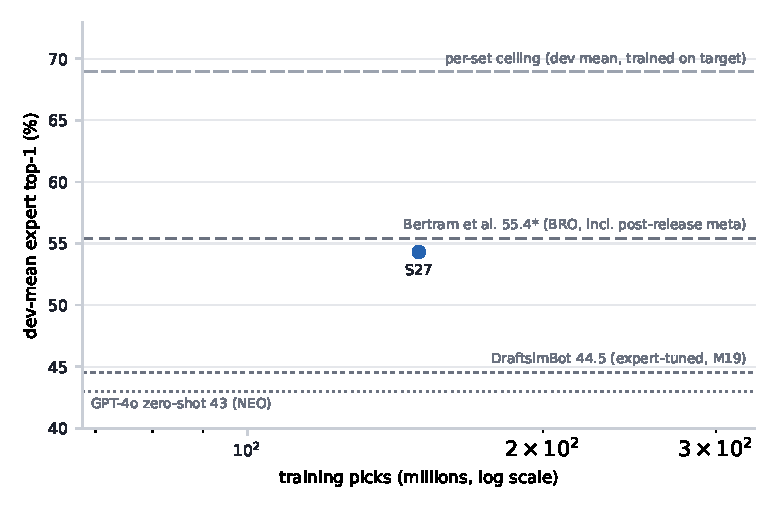
\includegraphics[width=0.78\linewidth]{figures/scaling_curve.pdf}
  \caption{Zero-shot dev-trio-mean top-1 agreement with high-win-rate
  players vs.\ training picks (log scale). Filled points: the nested
  scaling ladder; open points: set-composition probes. Horizontal rules
  mark published anchors and the per-set ceiling mean.}
  \label{fig:scaling}
\end{figure}

\begin{table}[t]
  \centering
  \caption{Scaling ladder. Rung labels are frozen protocol identifiers, not
  set counts: \emph{S27} names the top rung's run, which actually trains on
  28 sets, a naming artifact from an earlier corpus size, kept as-is rather
  than renamed after the fact. Set and pick counts in the table are the
  real values from run records. Dev-mean is the model-selection metric of
  \S\ref{sec:protocol}.}
  \label{tab:scaling}
  \small
  \setlength{\tabcolsep}{4pt}
  % AUTO-GENERATED by scripts/make_paper_tables.py -- do not edit.
% Scaling ladder (protocol section 4.3). Rung labels are frozen identifiers; counts come from run records.
\begin{tabular}{l p{4.8cm} rrrc}
\toprule
\rowcolor{tblhead}
Rung & Sets & \#sets & Train picks (M) & Best step & Dev-mean top-1 (\%) \\
\midrule
S1 & NEO & 1 & 5.4 & 4000 & 48.9 \\  % run=20260704_154741_s1; run=20260704_154741_s1
S2 & S1 + DSK & 2 & 13.3 & 18000 & 50.9 \\  % run=20260704_161450_s2; run=20260704_161450_s2
S2b & MOM, TDM (probe) & 2 & 14.5 & 8000 & 50.2 \\  % run=20260704_171827_s2b; run=20260704_171827_s2b
S4 & S2 + DMU, FIN & 4 & 27.8 & 24000 & 51.7 \\  % run=20260704_175554_s4; run=20260704_175554_s4
S4b & STX, SNC, OTJ, TLA (probe) & 4 & 23.5 & 20000 & 51.0 \\  % run=20260704_191659_s4b; run=20260704_191659_s4b
S8 & S4 + STX, MOM, BLB, TLA & 8 & 52.9 & 18000 & 52.4 \\  % run=20260704_202620_s8; run=20260704_202620_s8
S16 & S8 + AFR, SNC, ONE, LTR, WOE, MKM, OTJ, EOE & 16 & 99.9 & 34000 & 53.3 \\  % run=20260704_213310_s16; run=20260704_213310_s16
S27 & full F-dev universe & 28 & 149.4 & 34000 & 54.3 \\  % run=20260704_135822_f_dev; run=20260704_135822_f_dev
\bottomrule
\end{tabular}

\end{table}

\paragraph{Scaling.}
Figure~\ref{fig:scaling} and Table~\ref{tab:scaling} report zero-shot
accuracy as training grows from one set (NEO, 5.4M picks) to the full
\FdevSets-set universe (\FdevPicks M picks), under the fixed recipe.
Single-set training is the regime of \citet{bertram2024cards}'s
features-only anchor; the top rung is F-dev.
% Seed spread (within-training top-1, not a dev-trio zero-shot re-eval):
% run=20260704_154741_s1 (0.6824), run=20260705_170754_s1_seed18 (0.6774),
% run=20260705_170754_s1_seed19 (0.6768); run=20260704_175554_s4 (0.6892),
% run=20260705_170755_s4_seed18 (0.6881), run=20260705_170755_s4_seed19 (0.6880).
Two extra seeds at S1 and S4 give within-training top-1 spreads of
0.677--0.682 and 0.688--0.689. Training itself is not noise-dominated at
either rung; this checks in-distribution training stability and
complements the zero-shot dev-mean seed spread reported below.
% TODO-DRIVER: the literal seed-spread and composition-probe numbers in
% this paragraph and the next two (0.677-0.682, 0.688-0.689, 50.2, 50.9,
% 51.0, 51.7, pick counts) predate the macros-only rule; macro-ify if
% convenient. Values unchanged here.
% Log-linear fit of dev-mean top-1 on log2(train picks), nested ladder only
% (S1..F-dev/S27): scripts/analyze_scaling_shape.py, reading
% paper/figures/scaling_data.json (same source scaling_curve.py plots from).
% slope=1.037pp/doubling, R^2=0.980, max |residual|=0.43pp (S2). Per-segment
% doubling-normalized deltas: S1-S2 1.57, S2-S4 0.67, S4-S8 0.79, S8-S16
% 1.01, S16-F-dev 1.68 pp/doubling -- non-monotonic, no decay toward the
% top rung.
A log-linear fit of dev-mean top-1 on $\log_2$(training picks) across the
nested ladder (S1 through F-dev, 5.4M--149.4M picks) tracks the six rungs
closely: slope 1.0 percentage point per doubling, $R^2=0.98$, with no rung
off the fitted line by more than 0.4pp. But that same fit argues against
reading a diminishing-returns point into the tested range, not for one.
The per-doubling gain moves between 0.7 and 1.7pp/doubling, and it does so
non-monotonically: lowest across the S2--S8 middle of the ladder, highest
at the S1--S2 start and the S16--F-dev end, rather than decaying toward
the top rung.

Six error-bar-free points, on a fit whose own top rung is the model
selected on this axis, are not strong evidence of log-linearity. The
honest reading is narrower than it looks: no diminishing returns are
visible over the two orders of magnitude tested, which is not the same as
showing that returns do not saturate beyond that range.

Re-scoring those same extra-seed checkpoints on the zero-shot dev-mean the
curve actually plots, rather than on within-training top-1, gives
per-seed spreads of \SeedSpreadSone pp at S1 and \SeedSpreadSfour pp at
S4. That is at most about a quarter of the \SeedGainSoneSfour pp gain from
S1 to S4, so the rung-to-rung climb is not a seed artifact. These are
three-seed spreads at two rungs that also fold in an early-stop-step
difference (the two added seeds stopped at half the reference seed's
step), so they bound the curve's seed noise rather than fully characterize
it, standing in at S1/S4 as a proxy for the top rung.

The two composition probes offer a natural check on whether pick count
alone predicts a rung's score, or whether which sets are in it matters too.
At matched set count, S2b (MOM and TDM, 14.5M picks) scores 50.2\% against
S2's 50.9\%, despite having \emph{more} training picks than S2's 13.3M
(Table~\ref{tab:scaling}). If pick count were the whole story, S2b should
have scored higher, not lower. S4b (23.5M picks) scores 51.0\% against
S4's 51.7\%, in the direction pick count would predict, but S4 also has
more picks (27.8M), so that pair does not separate the two explanations.
Only S2 vs.\ S2b isolates set count from pick count, and on that one pair,
composition beats volume: which sets a rung trains on moves the score more
than how many picks they contribute. Two probe pairs is not enough to
generalize beyond that.
